\documentclass[12pt]{article}
\usepackage{geometry}                % See geometry.pdf to learn the layout options. There are lots.
\geometry{letterpaper}                   % ... or a4paper or a5paper or ... 
%\geometry{landscape}                % Activate for for rotated page geometry
%\usepackage[parfill]{parskip}    % Activate to begin paragraphs with an empty line rather than an indent
\usepackage{float}
\usepackage{graphicx}
\graphicspath{{images/}}
\usepackage{amsmath,amssymb,amsfonts,amsthm}
\usepackage{epstopdf}
\usepackage{cleveref}
\usepackage{epigraph}
\usepackage{url}
\usepackage{mathtools}

% Computer Concrete
%\usepackage{concmath}
%\usepackage[T1]{fontenc}

% Times variants
%
%\usepackage{mathptmx}
%\usepackage[T1]{fontenc}
%
%\usepackage[T1]{fontenc}
%\usepackage{stix}
%
% Needs to typeset using LuaLaTeX:
%\usepackage{unicode-math}
%\setmainfont{XITS}
%\setmathfont{XITS Math}

% garamond
%\usepackage[cmintegrals,cmbraces]{newtxmath}
%\usepackage{ebgaramond-maths}
%\usepackage[T1]{fontenc}

\DeclareGraphicsRule{.tif}{png}{.png}{`convert #1 `dirname #1`/`basename #1 .tif`.png}

\theoremstyle{plain}
\newtheorem{theorem}{Theorem}
\newtheorem{corollary}[theorem]{Corollary}
\newtheorem{lemma}[theorem]{Lemma}
\newtheorem{proposition}[theorem]{Proposition}
\newtheorem{conjecture}[theorem]{Conjecture}
\newtheorem{question}[theorem]{Question}
\newtheorem{definition}[theorem]{Definition}

\theoremstyle{definition}
\newtheorem{example}[theorem]{Example}
\newtheorem{todo}{TODO}

\theoremstyle{remark}
\newtheorem{remark}[theorem]{Remark}
\newtheorem{note}[theorem]{Note}

\title{Neural Networks Notes}
\author{Nhan Trong}
\date{July 6, 2016---\today}                                           % Activate to display a given date or no date

\begin{document}
\sloppy
\maketitle

\epigraph{Pipey. \textit{Looks like you want to compress a movie file, can I help? You know with Pied Piper's revolutionary neural network optimized sharded data distribution system, it's just six clicks away, follow meeee!}}{Silicon Valley}

\part{Different Types of Neurons and Learning}

\begin{question}
How many other neurons does a neuron talk to? Do they change neighbours?
\end{question}

\begin{note}
``Goal of unsupervised learning: provides a compact, low-dimensional representation of the input,'' like Pied Piper's compression algorithm using neural networks!
\end{note}

\section{Keywords}

Fruit flies, MNIST, TIMIT, linear, binary threshold, rectified / linear threshold, logistic, stochastic binary neurons, supervised, unsupervised, reinforcement learning.

\part{Neural Network Architectures}

\section{Keywords}

Feed forward, recurrent, symmetrically connected neural network, perceptrons, convexity condition.

\part{Perceptron Learning Algorithm}

\begin{todo}
Proof of why perceptron learning works is very sketchy! Need more details.
\end{todo}

\section{Binary Threshold Neurons McCulloch–Pitts}

Used in Perceptrons.

\begin{question}
Also called Linear Threshold Neurons?
\end{question}

\begin{definition}
First compute $z = w^T x$, then output $$y = \begin{cases}
1 \text{ if } z \geq 0 \\
0 \text{ otherwise,}
\end{cases}$$ representing ``all VS none'' activation.
\end{definition}

\begin{note}
Here we implicitly added the threshold as a bias unit: $w = (b, w_1, w_2, \ldots)$.
\end{note}

\begin{remark}
The function $y(z)$ is also called the Heaviside / unit step function.
\end{remark}

\begin{figure}[H]
\centering
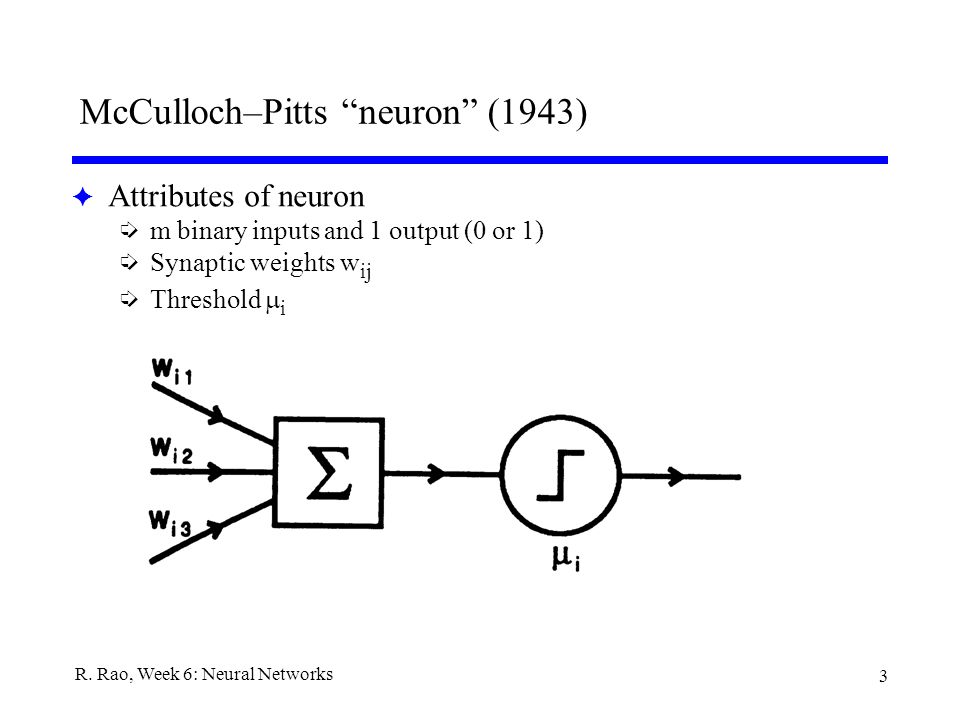
\includegraphics[width=1.0\textwidth]{mccullochpitts}
\end{figure}

\section{Limitations of the Binary Threshold Neuron}

\begin{proposition}
A single binary threshold neuron cannot learn the XOR function, because geometrically its truth table represented on a plane is not linearly separable.
\end{proposition}

\begin{figure}[H]
\centering
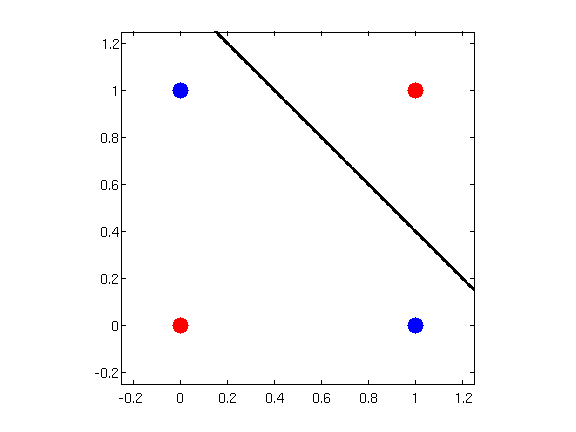
\includegraphics[width=1.0\textwidth]{linSepXor}
\end{figure}

\subsection{Group Invariance Theorem}

\begin{proposition}
Perceptrons can't learn patterns if they're subject to transformations that form a group, e.g. translations with wrap-around.
\end{proposition}

\begin{question}
Details?
\end{question}

\section{Keywords}

Data space, weight space, Group Invariance Theorem.

\part{Linear Neuron Learning Algorithm}

\begin{definition}
Given a training case $x_n$ and a weight vector $w$, the neuron's estimate $y_n$ of the desired output is $$y_n = \sum_{i}^{} w_i x_{ni} = w^T x_n.$$ Define the cost function $E_n$ to be the squared difference error $$E_n = \frac{1}{2}(t_n - y_n)^2,$$ where $t_n$ is the target output, i.e. the ``ground truth'', and define the total error to be $$E = \sum_{n}^{} E_n.$$ Finally the goal of learning is to minimize $E$: $$\min_{w} E.$$
\end{definition}

\section{Delta Rule: Learning by Gradient Descent}

The error partials are 
$$\frac{\partial E}{\partial w_i} = \sum_n \frac{dE_n}{dy_n} \frac{\partial y_n}{\partial w_i} = - \sum_n (t_n - y_n) x_{ni}.$$
The Delta Rule / Gradient Descent says that we should change $w_i$ in the opposite direction as the change in error along $w_i$, give or take a learning rate $\alpha$:
$$\Delta w_i = - \alpha \frac{\partial E}{\partial w_i} = \sum_n \alpha (t_n - y_n) x_{ni},$$ i.e. $\alpha$ tells us how much to change, and the negative sign tells us which direction to go, namely the opposite direction. E.g. if $\frac{\partial E}{\partial w_i} > 0,$ that means the error goes up as $w_i$ increases, so we want to decrease $w_i$ to make it go down, and vice versa.

\section{Error Surface of a Linear Neuron}

\begin{question}
IIRC feature normalization should help with slow learning due to unscaled data? What about pathological cases like this, called the Rosenbrock Valley?
\end{question}

\begin{figure}[H]
\centering
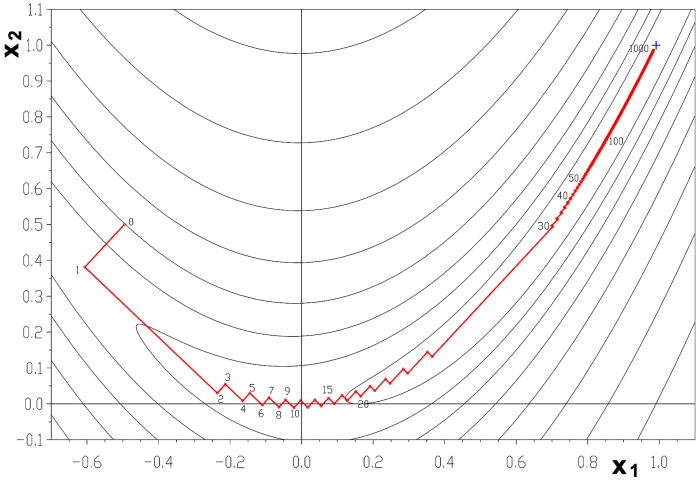
\includegraphics[width=1.0\textwidth]{slowlearrning}
\end{figure}

\section{Keywords}

Linear neurons / linear filters, iterative / computational VS analytic / mathematical approach, Delta Rule / Gradient Descent, batch VS online, error surface, extended weight space, Rosenbrock function.

\part{Logistic Neurons}

\section{Learning Rule}

\begin{definition}
The estimator for a logistic neuron is given by
$$y = \frac{1}{1 + e^{-z}}$$ where $z = w^T x.$ The function $y(z)$ is also known as a logistic / sigmoid function, and $z$ is sometimes called the logit. As before, the error is the squared difference
$$E = \frac{1}{2} \sum_n (t_n - y_n)^2.$$
\end{definition}

\begin{proposition}
The estimator derivatives are
$$\frac{\partial y}{\partial w_i} = \frac{dy}{dz} \frac{\partial z}{\partial w_i} 
= y(1 - y) x_i,$$ and so the error derivatives are
$$\frac{\partial E}{\partial w_i} = \sum_n \frac{dE_n}{dy_n} \frac{\partial y_n}{\partial w_i} = - \sum_n (t_n - y_n)(1 - y_n) y_n x_{ni}.$$
\end{proposition}

\section{Learning with Hidden Units}



\section{Backpropagation Algorithm}



\section{Keywords}

Sigmoid function, logit, Backpropagation Algorithm.

\begin{thebibliography}{99}

\bibitem{hinton}
Geoffrey E. Hinton's Neural Networks video lectures.

\bibitem{csc321}
\url{http://www.cs.toronto.edu/~rgrosse/csc321/}

\end{thebibliography}

\end{document}
